\documentclass[tikz]{standalone}

    \usetikzlibrary{shapes}
    \usetikzlibrary{circuits.ee.IEC}
    \usetikzlibrary{angles, math, calc, matrix}
    \usetikzlibrary{decorations.pathreplacing, decorations.markings,calligraphy}

\begin{document}
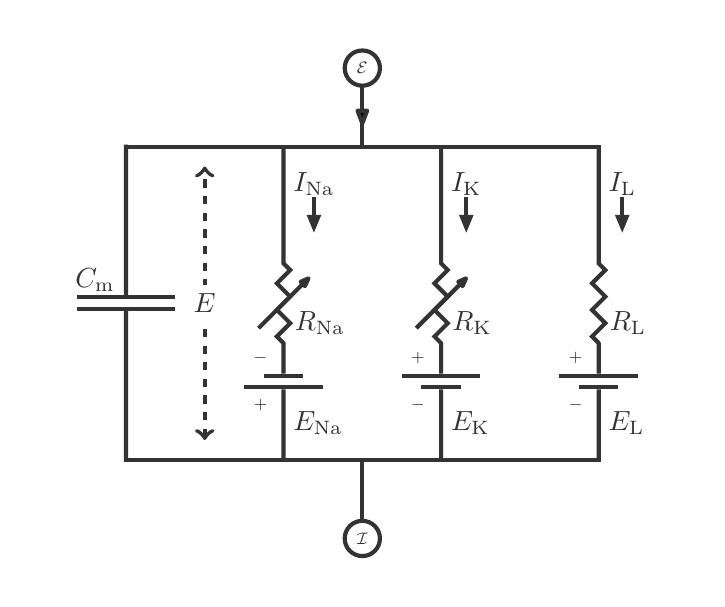
\begin{tikzpicture}[
    %x=1cm, y=1cm, 
    %z={(0cm,1cm)},
    scale = 1,
    line width = 1.5pt, 
    black!80,
    circuit ee IEC,
    every info/.style={font=\footnotesize},
        small circuit symbols,
            set resistor graphic=var resistor IEC graphic,
            set diode graphic=var diode IEC graphic,
            set make contact graphic= var make contact IEC graphic
    ]

    % Determines the boundries
    \path [use as bounding box] (-4.25,-3.5) rectangle (4.25,3.5);

    
    \def\r{0.5}
    \def\l{2}
    \def\w{0.5}
    \def\j{2cm}
    \def\chanGap{3cm}
    \def\exShift{3}
    \def\s{0.5}
    \def\steps{4}
    
    % Ratio for each ion
    \def\Nar{1/3}
    \def\Kr{2/3}
    \def\Lr{3/3}
    \def\Nas{Na}
    %\def\Kr{3/12}
    %\def\Nar{7/12}
    %\def\Nar{1/(2*\r*\s)}
    \def\Clr{11/12}

    \def\boxRatio{33.50}
    \def\boxSize{3.6}
    
    \def\pcoord#1{{#1:\boxSize}}

    \coordinate (O) at (0,0);
    \coordinate (TR) at (\pcoord{\boxRatio});
    \coordinate (TL) at (\pcoord{180-\boxRatio});
    \coordinate (BL) at (\pcoord{180+\boxRatio});
    \coordinate (BR) at (\pcoord{-\boxRatio});

    
    % Outlining the circutry
    \draw[line width = 0.5] (TL) -- (TR)++(-0.75,0) (BL) -- (BR)++(-0.75,0);
    \draw ($(TL)!1/2!(TR)$) -- ++(0,1) node (E) [scale = 0.75,circle,draw,fill = white] {\footnotesize $\mathcal{E}$}
          ($(BL)!1/2!(BR)$) -- ++(0,-1) node (I) [scale = 0.75,circle,draw,fill = white] {\footnotesize $\mathcal{I}$};

    \draw (E) to [current direction] ($(TL)!1/2!(TR)$);
    
    
    \draw[line cap = rect] (TL) -- (TR) (BL) -- (BR);


    % Leakage of potential
    \draw[line cap = rect]  (BL) to [capacitor={minimum height=1.25cm, minimum width=0.15cm}] (TL);
    \path (BL) -- (TL) node[midway, anchor = south east] {$C_\mathrm{m}$};

    
    \foreach \f/\i/\r/\a in 
        {\Nar/Na/0/adjustable', \Kr/K/180/adjustable', \Lr/L/180/}{
        % Making the main circuit paths
        \draw ($(BL)!\f!(BR)$) to  [battery={near start,minimum height=1cm, minimum width=0.15cm, rotate = \r}, resistor={\a}] node[right, yshift = -0.25cm]{$R_\mathrm{\i}$} ($(TL)!\f!(TR)$);  

        % Making external markings
        \path ($(TL)!\f!(TR)$) -- ($(BL)!\f!(BR)$) node (I\i) [ near start, anchor = south west, fill = white,inner sep=0pt, xshift = 0.1cm, yshift = 0.35cm]  {$I_{\mathrm{\i}}$};
        
        \path ($(TL)!\f!(TR)$) -- ($(BL)!\f!(BR)$) node (E\i) [ near end, anchor = north west, fill = white, inner sep=0pt, xshift = 0.1cm, yshift = -0.35cm]  {$E_{\mathrm{\i}}$};

        \foreach \o in {-,+}{
            \path ($(TL)!\f!(TR)$) -- ($(BL)!\f!(BR)$) node (S\i\o) [ near end, anchor = east, fill = white, inner sep=0pt, xshift = -0.25cm, yshift = \o 0.30 cm]  {};
        }
    }

    \path ($(BL)!1/6!(BR)$) -- +(0, 0.25) coordinate (BE)
          ($(TL)!1/6!(TR)$) -- +(0,-0.25) coordinate (TE);
    \draw[dashed, <->] (BE) -- (TE) node[midway,fill=white] {$E$};


    \foreach \i in {Na,K,L}{
        \draw (I\i) -- +(0,-0.45cm) 
        node[isosceles triangle, scale = 0.25, draw, fill, rotate = 270] 
        {};
        \ifx\i\Nas
            \foreach \o/\s in {-/+,+/-}{
                 \path (S\i\o) node {\tiny $\s$};
        }
        \else
            \foreach \o in {-,+}{
                 \path (S\i\o) node {\tiny $\o$};
        }
        \fi
    }
    

        
\end{tikzpicture}
\end{document}